% !TEX root = ../../../main.tex
% 来源：中学数学实验教材·第三册（高中数学）
% 章节：任意角的三角函数 / 三角函数的诱导公式
% 原始文件：6.tex，行 2002-2014
% 类型：tikz
% ---
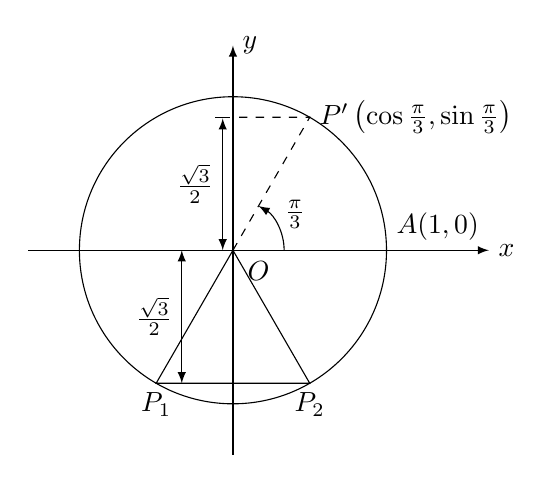
\begin{tikzpicture}[>=latex, scale=1.3]
    \draw[->](-2,0)--(2.5,0)node[right]{$x$};
    \draw[->](0,-2)--(0,2)node[right]{$y$};
    \draw (0,0) circle(1.5);
\draw (0,0)--(.75,-.75*1.732)node[below]{$P_2$}--(-.75,-.75*1.732)node[below]{$P_1$}--(0,0);
\draw[dashed] (0,0)--(60:1.5)node[right]{$P'\left(\cos\frac{\pi}{3},\sin\frac{\pi}{3}\right)$}--(0,.75*1.732);
\node at (2,0)[above]{$A(1,0)$};
\draw[->](.5,0) arc (0:60:.5);
\node at (30:.7){$\frac{\pi}{3}$};
\draw[|<->] (-.1,.75*1.732)--node[left]{$\frac{\sqrt{3}}{2}$}(-.1,0);
\draw[<->] (-.5,-.75*1.732)--node[left]{$\frac{\sqrt{3}}{2}$}(-.5,0);
\node at (.25,-.2){$O$};
\end{tikzpicture}
